\documentclass[../../master-handout.tex]{subfiles}

\begin{document}

\section{Lecture 4 (Thu, May 21)}
\sidenote{\textbf{Scribe:} Junzhang Luo \\ \textbf{Date:} Thu, May 21, 2026}

\subsection{Representations of Rotations}

A rotation in three-dimensional space has three degrees of freedom. Several common ways to represent rotations are:

\begin{enumerate}
    \item \textbf{Euler angles}, such as the ZYZ convention.
    \item \textbf{Roll-pitch-yaw (RPY) angles}.
    \item \textbf{Axis-angle representation}, using a unit axis
    \[
        k = (k_x, k_y, k_z), \qquad \|k\| = 1,
    \]
    together with a rotation angle \(\theta\).
    \item \textbf{Unit quaternions}, represented by four numbers:
    \[
        Q =
        \left(
            \cos{\frac{\theta}{2}},
            k_x \sin{\frac{\theta}{2}},
            k_y \sin{\frac{\theta}{2}},
            k_z \sin{\frac{\theta}{2}}
        \right).
    \]
\end{enumerate}

\sidenote{Euler angles and RPY angles are minimal because they use three parameters, but they can have singularities. Unit quaternions are not minimal, since they use four numbers with a unit-norm constraint.}

A homogeneous transformation matrix \(H_n^0(q)\) represents the pose of frame \(n\) relative to frame \(0\). It contains both a rotation and a translation:
\[
    H_n^0(q) \in SE(3) \subset \mathbb{R}^{4 \times 4}.
\]
The group \(SE(3)\), called the special Euclidean group, is the set of rigid body motions in three dimensions.

For example, if \(\bar{p}^2\) is a point written in homogeneous coordinates in frame \(2\), then
\[
    H_1^0 H_2^1 \bar{p}^2
    =
    H_1^0 \bar{p}^1
    =
    \bar{p}^0
    =
    H_2^0 \bar{p}^2,
\]
where
\[
    H_2^0 = H_1^0 H_2^1.
\]

The \textbf{direct kinematics map} is
\[
    H_n^0 : q \mapsto H_n^0(q),
    \qquad
    \mathbb{R}^n \to SE(3).
\]
For a serial manipulator,
\[
    H_n^0(q)
    =
    H_1^0(q_1)
    H_2^1(q_2)
    \cdots
    H_n^{n-1}(q_n).
\]

\subsection{Denavit--Hartenberg Parameters}

The Denavit--Hartenberg convention gives a systematic way to assign coordinate frames to links and joints.

For the link between joint \(i-1\) and joint \(i\), define a reference frame
\[
    o_{i-1}x_{i-1}y_{i-1}z_{i-1}.
\]
The \(z_{i-1}\)-axis is chosen along the axis of joint \(i\), while the \(x\)-axis is chosen along the common normal between consecutive joint axes.

\begin{fullwidth}
\begin{figure}
    \centering
    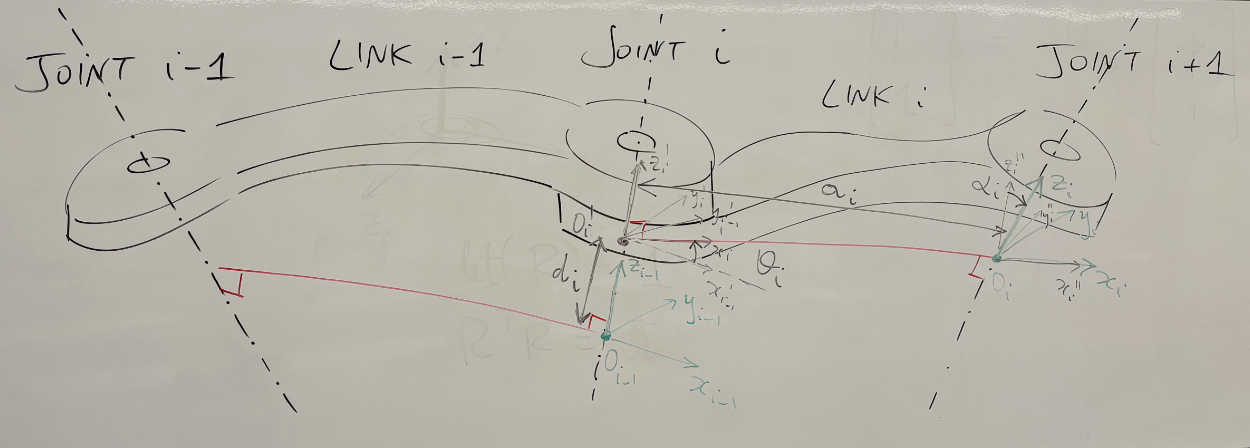
\includegraphics[width=0.75\linewidth]{./lecture-4img/05-21-joint.png}
    \caption{Reference frame assignment for consecutive joints under the Denavit--Hartenberg convention.}
\end{figure}
\end{fullwidth}

To move from frame \(i-1\) to frame \(i\), we use four transformations:

\begin{enumerate}
    \item Translate by \(d_i\) along \(z_{i-1}\).
    \item Rotate by \(\theta_i\) about \(z_{i-1}\).
    \item Translate by \(a_i\) along \(x_i\).
    \item Rotate by \(\alpha_i\) about \(x_i\).
\end{enumerate}

The four DH parameters are:

\begin{itemize}
    \item \(d_i\): offset along \(z_{i-1}\).
    \item \(\theta_i\): rotation angle about \(z_{i-1}\).
    \item \(a_i\): link length along the common normal.
    \item \(\alpha_i\): twist angle about \(x_i\), aligning \(z_{i-1}\) with \(z_i\).
\end{itemize}

\sidenote{For a revolute joint, \(\theta_i\) is the joint variable. For a prismatic joint, \(d_i\) is the joint variable. The remaining DH parameters are fixed by the robot geometry.}

Using the standard DH convention, the homogeneous transformation is
\[
    H_i^{i-1}(q_i)
    =
    R_z(\theta_i)T_z(d_i)T_x(a_i)R_x(\alpha_i).
\]

In matrix form,
\[
    H_i^{i-1}(q_i)
    =
    \begin{bmatrix}
        c_{\theta_i} & -s_{\theta_i} & 0 & 0 \\
        s_{\theta_i} & c_{\theta_i} & 0 & 0 \\
        0 & 0 & 1 & d_i \\
        0 & 0 & 0 & 1
    \end{bmatrix}
    \begin{bmatrix}
        1 & 0 & 0 & a_i \\
        0 & c_{\alpha_i} & -s_{\alpha_i} & 0 \\
        0 & s_{\alpha_i} & c_{\alpha_i} & 0 \\
        0 & 0 & 0 & 1
    \end{bmatrix}.
\]

Multiplying these matrices gives
\[
    H_i^{i-1}(q_i)
    =
    \begin{bmatrix}
        c_{\theta_i}
        & -s_{\theta_i}c_{\alpha_i}
        & s_{\theta_i}s_{\alpha_i}
        & a_i c_{\theta_i}
        \\
        s_{\theta_i}
        & c_{\theta_i}c_{\alpha_i}
        & -c_{\theta_i}s_{\alpha_i}
        & a_i s_{\theta_i}
        \\
        0
        & s_{\alpha_i}
        & c_{\alpha_i}
        & d_i
        \\
        0 & 0 & 0 & 1
    \end{bmatrix}.
\]

\subsection{Non-Uniqueness of the DH Convention}

The DH convention is useful, but the frame assignment is not always unique. Non-uniqueness can occur in the following cases:

\begin{enumerate}
    \item The base frame, since there is no previous link.
    \item The end-effector frame, since there is no next link.
    \item Parallel consecutive joint axes.
    \item Intersecting consecutive joint axes.
    \item Prismatic joints.
\end{enumerate}

\sidenote{If consecutive joint axes are parallel, there are infinitely many possible common normals. If they intersect, the common normal has zero length, so the frame assignment can become ambiguous.}

For prismatic joints, the displacement \(d_i\) changes with the joint variable, rather than the angle \(\theta_i\). Therefore, extra care is needed when identifying which DH parameter is variable.

\end{document}